\begin{frame} \frametitle{Results: Growth of the interface perturbation}
  % \vspace*{-0.25cm}%
  % \hspace*{0.03\textwidth}%
  % \begin{minipage}{0.2\linewidth}
  %   \hfill%
  %   \begin{figure}
  %     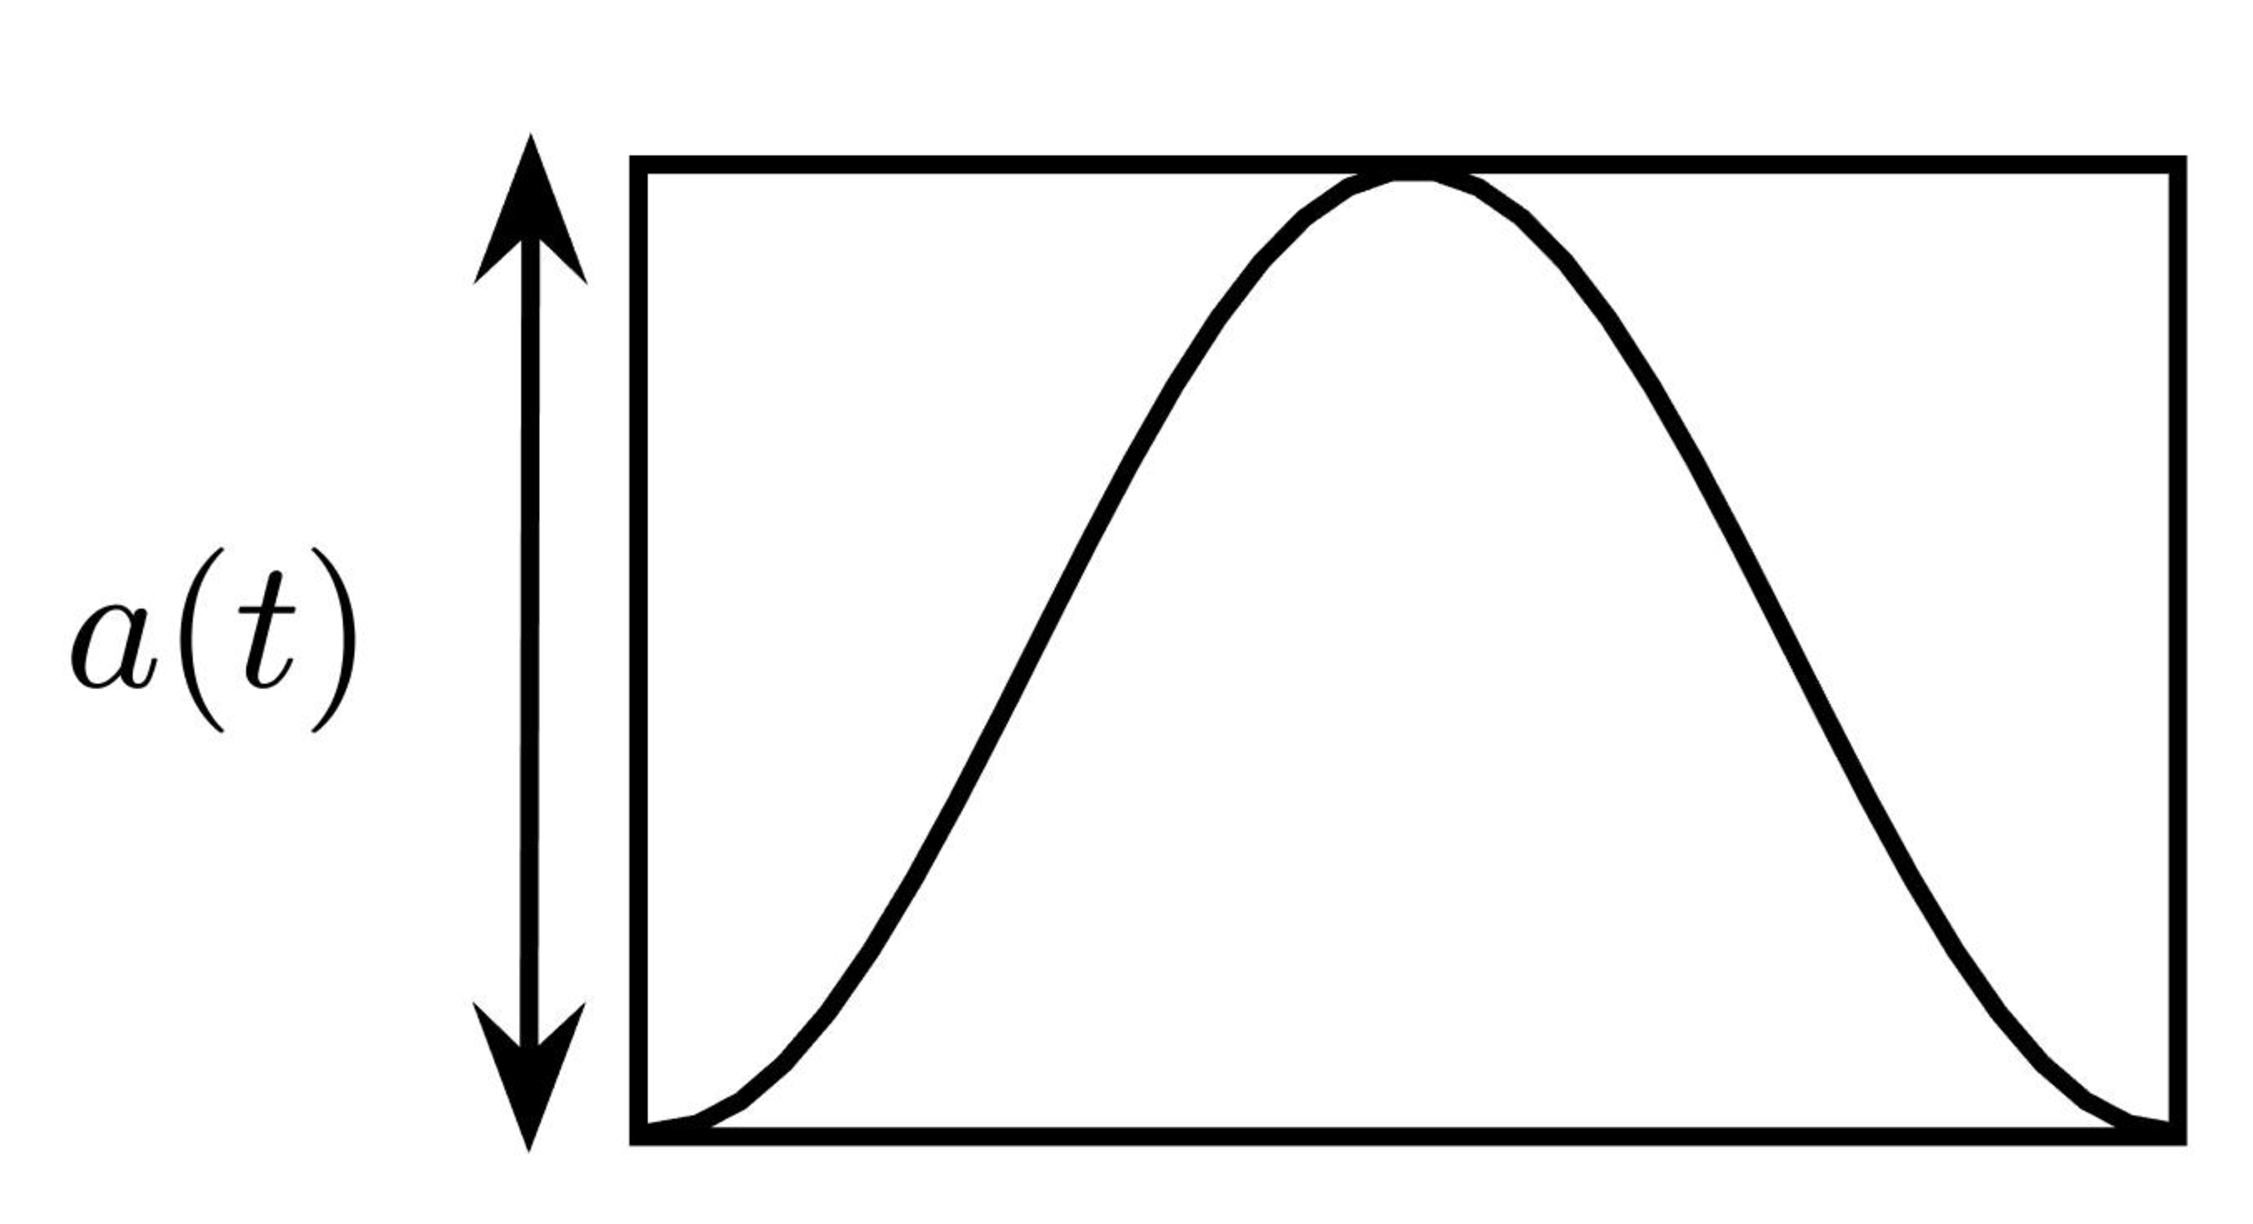
\includegraphics[height=0.18\textheight]{../figs/lung_figs/a0_schematic}%
  %   \end{figure}
  % \end{minipage}
\begin{figure}
  % \hfill%
  \centering
  % 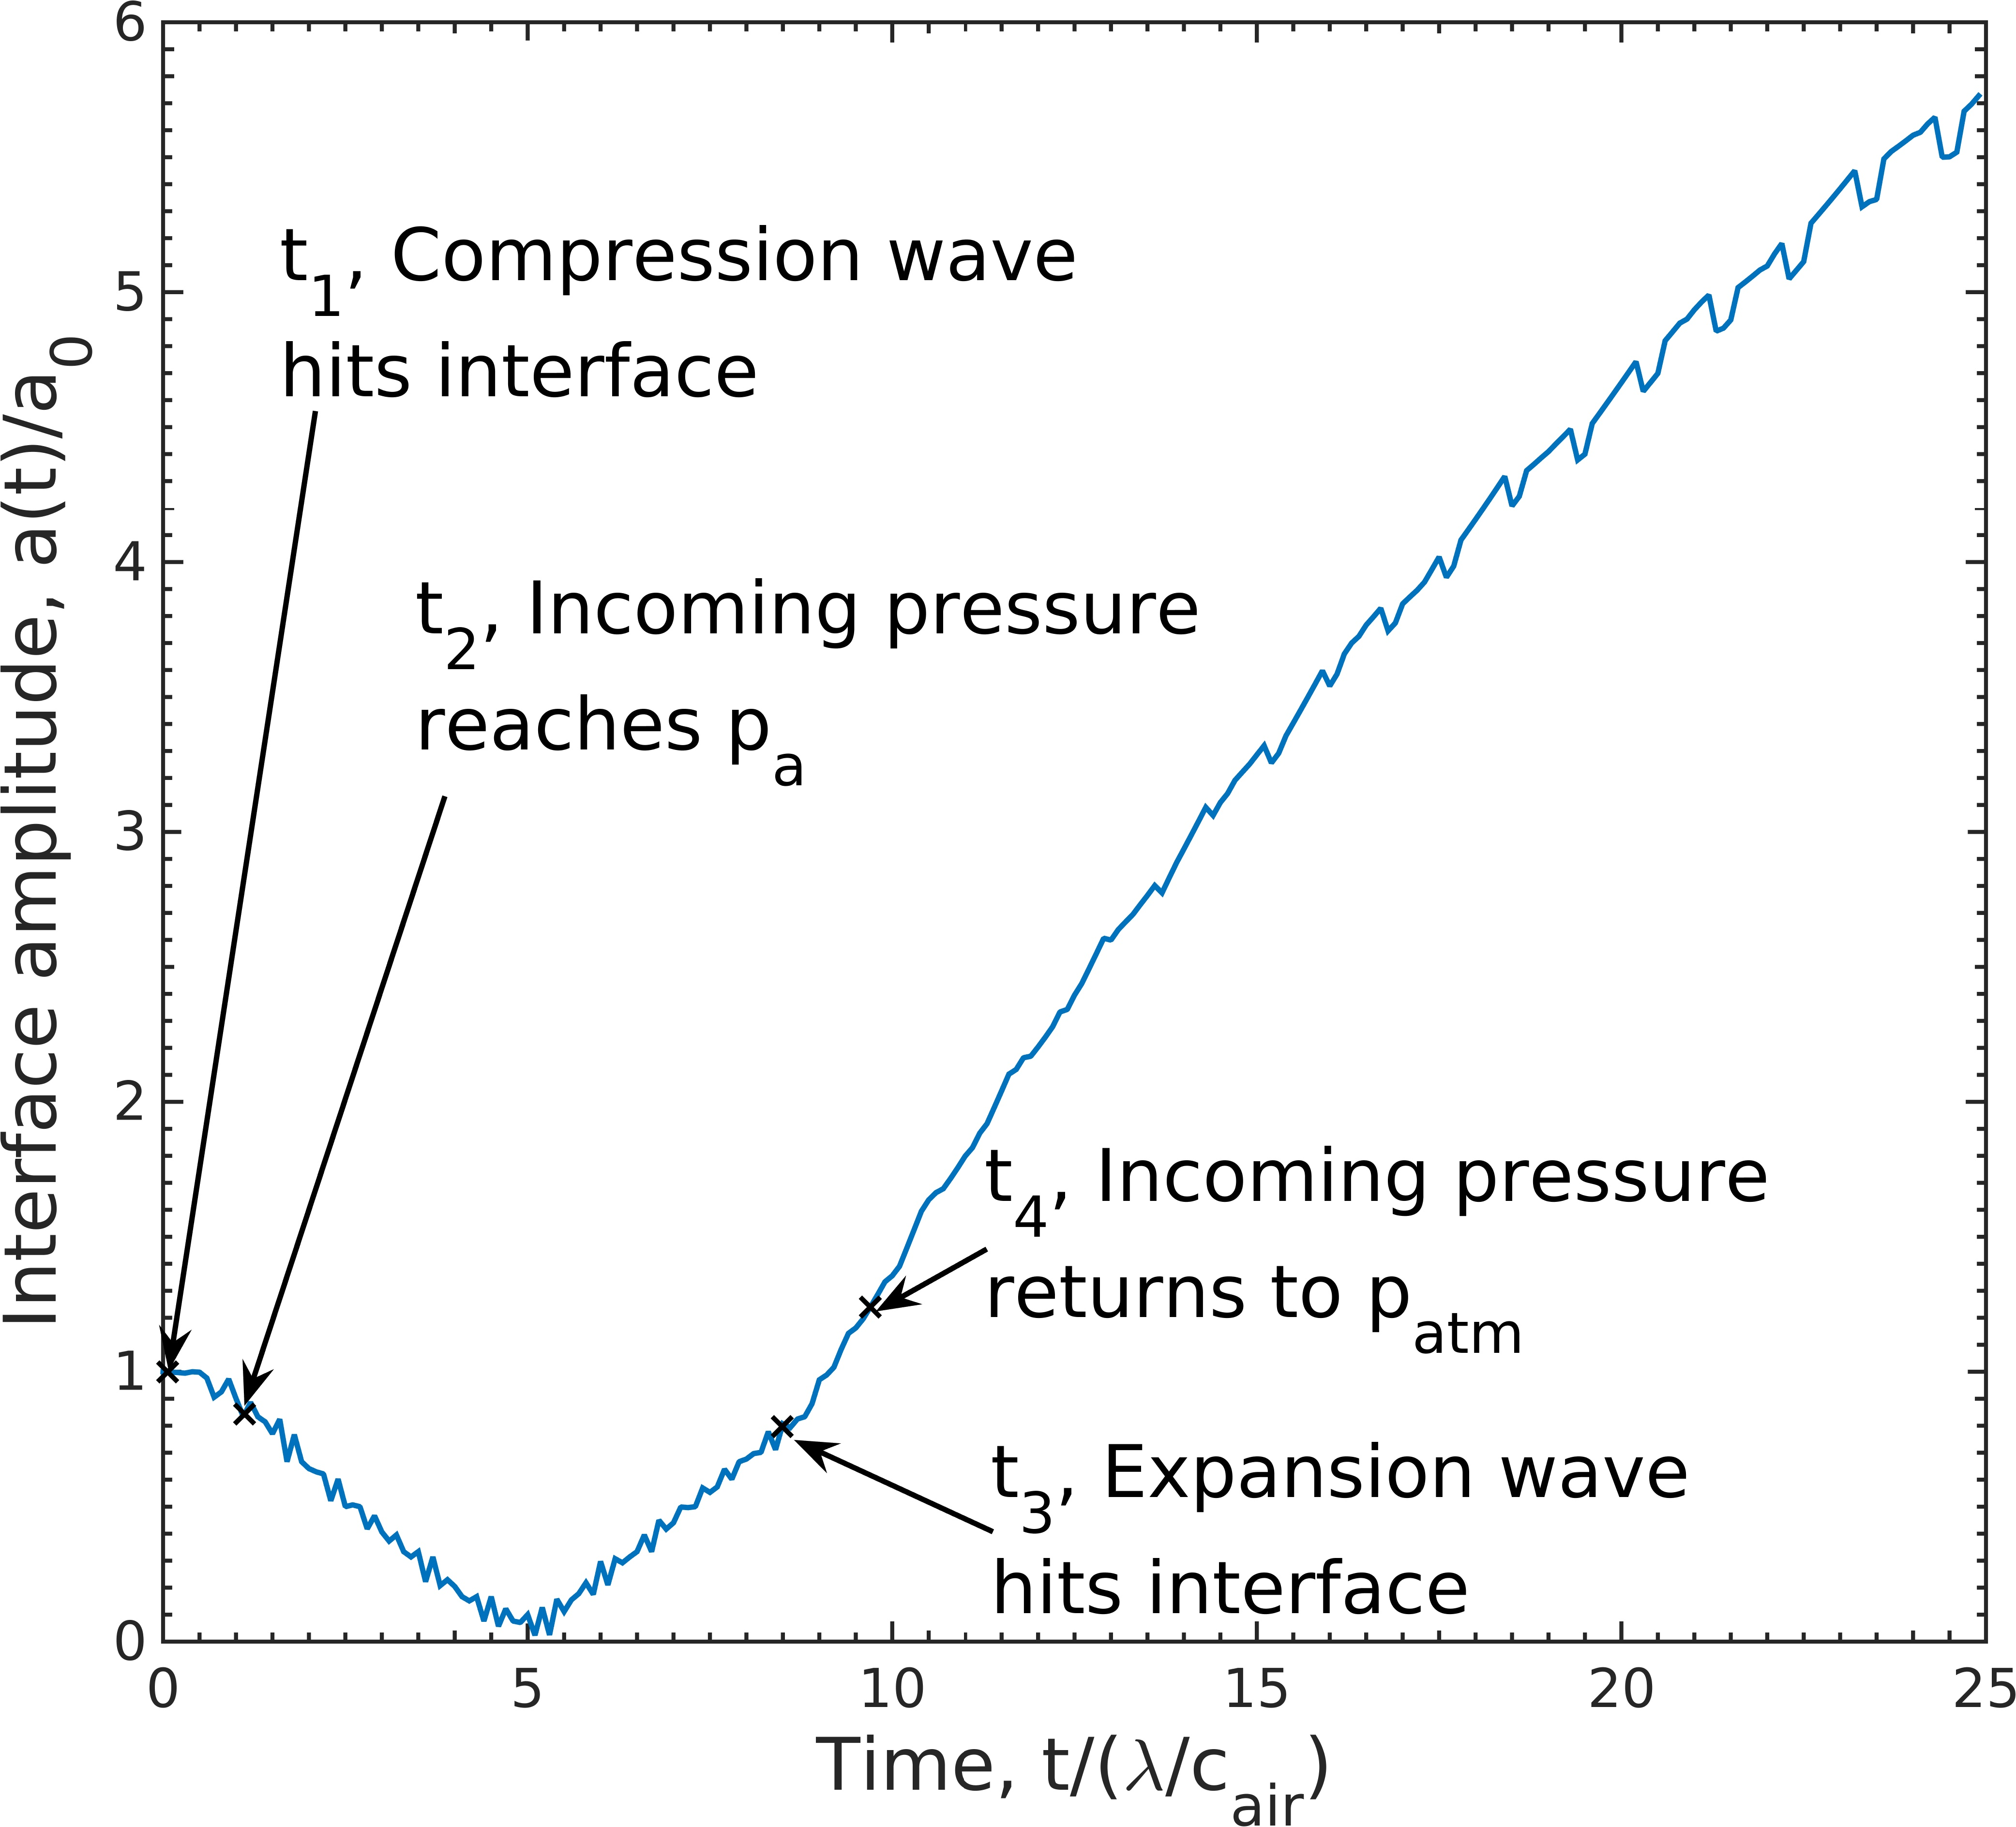
\includegraphics[height=0.5\textheight]{../figs/lung_figs/trapz10_intf_schematic}%
  \begin{subfigure}{0.48\textwidth}
    \begin{tikzpicture}
      \node[anchor=south west,inner sep=0] (image) at (0,0) {%
        \includegraphics[height=0.5\textheight]{./figs/trapz10_intf_schematic_24-May-2017}%
      }; \node[anchor=south west,inner sep=0] (image) at (0.5,3.0)
      {%
        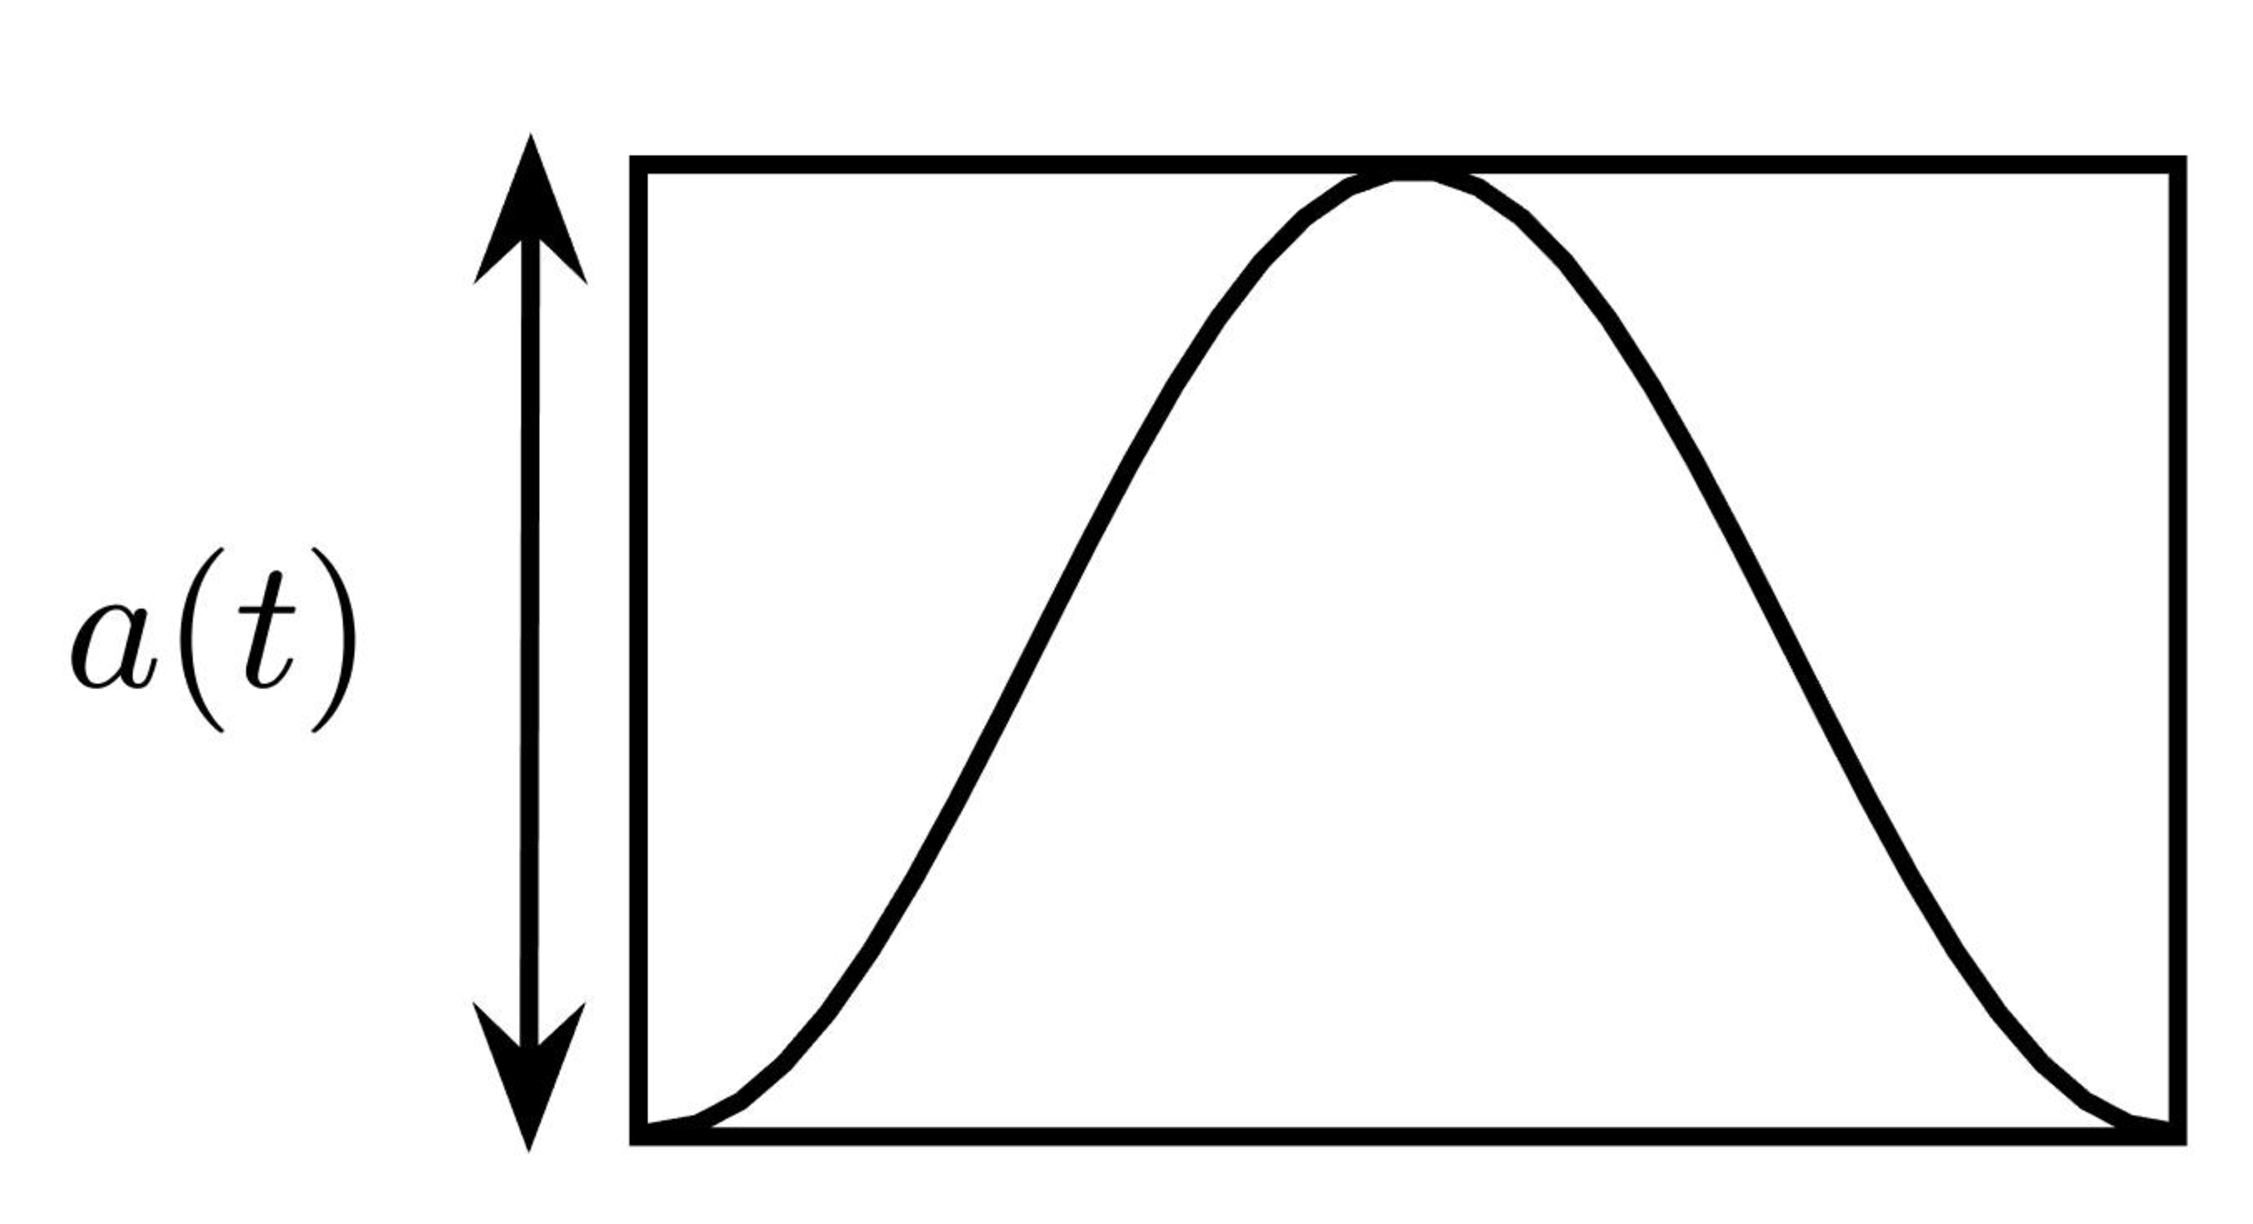
\includegraphics[height=0.15\textheight]{../figs/lung_figs/a0_schematic}%
      };
    \end{tikzpicture}
  \end{subfigure}
  \begin{subfigure}{0.48\textwidth}
    \begin{tikzpicture}%
      \node[anchor=south west,inner sep=0] (image) at (0,0) {%
        \includegraphics<1>[height=0.5\textheight]{../figs/lung_figs/p0_vs_t}%
        \includegraphics<2>[height=0.5\textheight]{./figs/trapz10_intf_t1000_24-May-2017}%
      };%
      \only<1>{
      \begin{scope}[x={(image.south east)},y={(image.north west)}]%
        \node[font=\footnotesize,right] at (0.22,0.18){ $t_1$};%
        \node[font=\footnotesize,right] at (0.22,0.8){ $t_2$};%
        \node[font=\footnotesize,right] at (0.83,0.8){ $t_3$};%
        \node[font=\footnotesize,right] at (0.82,0.18){ $t_4$};%
      \end{scope}%
      }
    \end{tikzpicture}%
  \end{subfigure}
\end{figure}
\only<1>{%
  The interface perturbation is initially compressed: $0^+\leq t/(\ell/c)\leq24$; experiences a phase change at $t/(\ell/c)\approx24$, then grows: $t/(\ell/c)>24$.%
}%
\only<2>{
  The interface perturbation continues to grow at late times, long after the wave has passed. Eventually, the growth appears asymptotic.%We suspect vorticity.%
}
  %
  \note{
    \begin{enumerate}
    \item A: Compression during wave,\\B: stretching after,\\T: Not linear acoustics, power-law growth
    \item If we look at the peak-to-peak amplitude of the interface
      perturbation as a function of time, we can see that early own
      the interface compresses slightly during the compression wave
    \item Then continues to compress until inverting phase at $t=5$.
    \item After the phase inversion, the expansion occurs.
    \item And the interface continues growing long after the wave has completely left.
    \end{enumerate}
  }
\end{frame}
%%% Local Variables:
%%% mode: latex
%%% TeX-master: "../main"
%%% End:
